\chapter{Detekce světelných stop v obraze}
\label{sec:detection}
Pro analýzu vlastností broušeného kamene je důležité detekovat světelné stopy vzniklé dopadem laserových svazků na stínítko. Zároveň je třeba určit parametry stop, které se budou porovnávat s parametry svazků matematického modelu kamene. 

Intenzitu pixelu $I$ můžeme vyjádřit jako 
\begin{equation}
	I = I_{beam}+I_{back}+I_{edge}+I_{\varepsilon}\,,
	\label{eq:intensitu_sum}
\end{equation}
 kde $I_beam$ reprezentuje příspěvek světelného svazku, $I_{back}$ intenzitu pozadí, $I_{edge}$ intenzitu světelných ocásků a $I_{\varepsilon}$ Poissonův šum (kapitola \ref{sec:poisson}). Jedním z úkolů detektoru je oddělit pozadí od zbývajících složek intenzit. Po odečtení pozadí získáme obrazy laserových svazků.   
 
Jednoduchým postupem pro určení intenzity pozadí by bylo prahování obrazu nad konstantní úrovní. V našem obraze však typicky konstantní není (kapitola \ref{sec:stinitko}). 

Rozdílné pozadí se může také vytvořit odrazem zdrojového svazku od jiných předmětů, než broušeného kamene. Hlavním příspěvkem je v tomto případě odraz od podstavce, na který pokládáme broušený kámen (obr. \ref{fig: podstavec}).

\begin{figure}[htps]
\centering
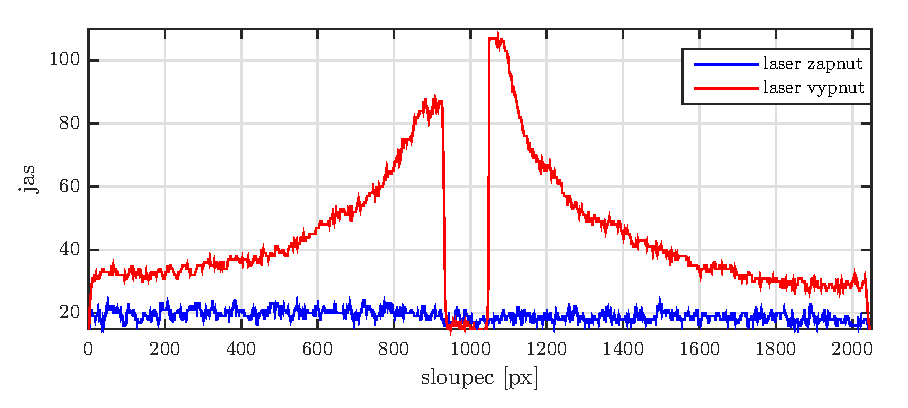
\includegraphics[width = 0.7\textwidth]{podstavec.eps}
\caption{Jasové úrovně ve vybraném řádku obrazu. Řádek protíná obraz podstavce. V případě červené charakteristiky dopadá na podstavec laserový svazek, rozptyluje se dopadá na stínítko. Modrou charakteristiku pozorujeme, pokud je laser vypnutý.}
\label{fig: podstavec}
\end{figure}

Hodnotu pozadí potřebujeme znát, abychom ze snímku mohli spočítat světelný tok pro jednotlivé dopadající laserové svazky. Určení intensity pozadí v každém pixelu komplikují obraz podstavce na kámen a okolí stínítka. Zde je intenzita světla podstatně nižší, než na povrchu stínítka. Vysoká změna jasu v obraze komplikuje určení pozadí.  

V okolí stínítka můžeme detekovat falešné svazky, které je třeba odstranit. 

Světelné stopy se mohou překrývat. Pro odlišení příspěvků jednotlivých svazků je třeba obraz prahovat v několika úrovních jasu.

V místě, kde je vysoká koncentrace svazků mohou dokonce svazky dopadnout tak blízko sebe, že splynou v jednu stopu (obr. \ref{Splynuti}).  

\begin{figure}[htbp]
    \centering
    \begin{minipage}[c]{0.48\textwidth}
        \centering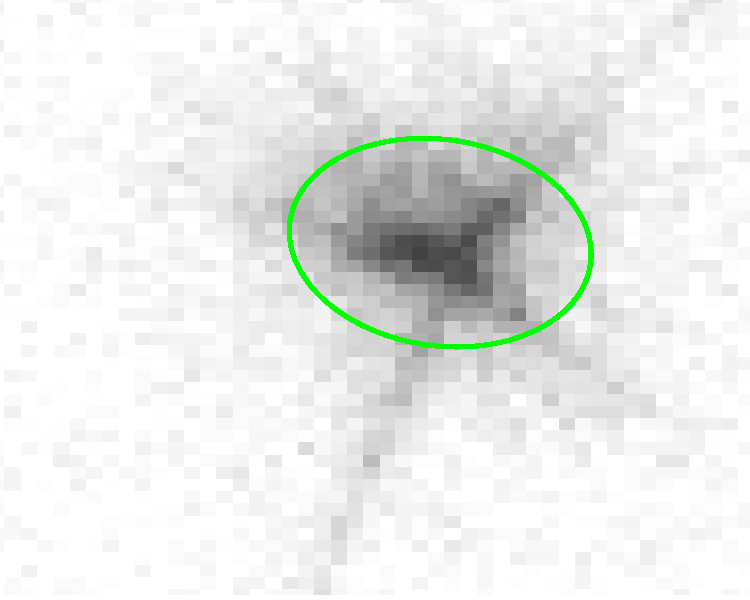
\includegraphics[width=.5\textwidth]{pf_near.pdf}
    \end{minipage}
    \begin{minipage}[c]{0.48\textwidth}
        \centering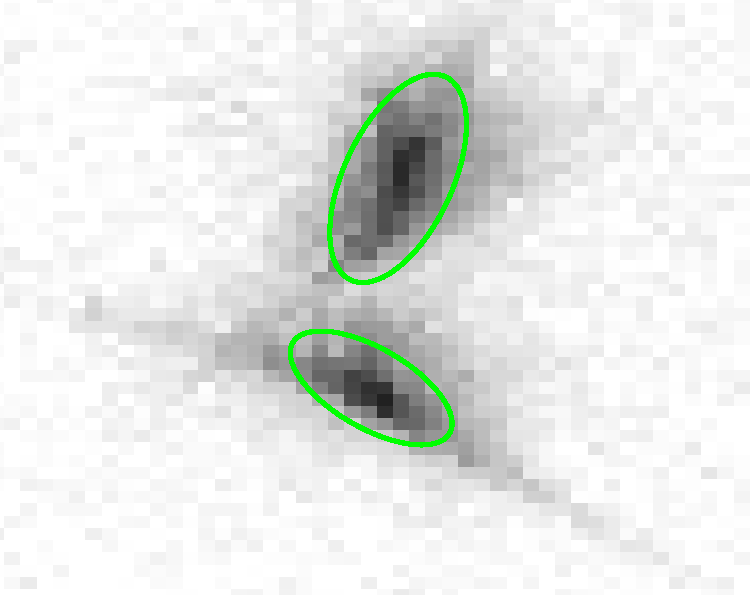
\includegraphics[width=.5\textwidth]{pf_near2.pdf}
    \end{minipage}
    \\
        \caption[Slynutí dvou různých svazků.]{Ilustrace slynutí dvou různých svazků. V pravém i levém snímku se nachází typově stejné laserové svazky. Na levém obrázku dopadly na stínítko příliš blízko sebe. V tomto případě nejsme schopni rozlišit příspěvek obou svazků a detekujeme pouze jednu stopu.}
        \label{Splynuti}
\end{figure}

Obraz je třeba filtrovat. Filtrováním snížíme šum v odraze, ale zároveň zmenšíme kontrast mezi stopami. 

Ne všechny svazky vystupující z kamene je možné detekovat. Svazky s vícenásobným odrazem postupně ztrácí zářivý tok. Po dopadu na stínítko mohou být nerozlišitelné od šumu a jejich detekce je prakticky nemožná. Pro stopy s nízkým jasem bude detekce často selhávat

\begin{figure}[htbp]
    \centering
    \begin{minipage}[c]{0.48\textwidth}
        \centering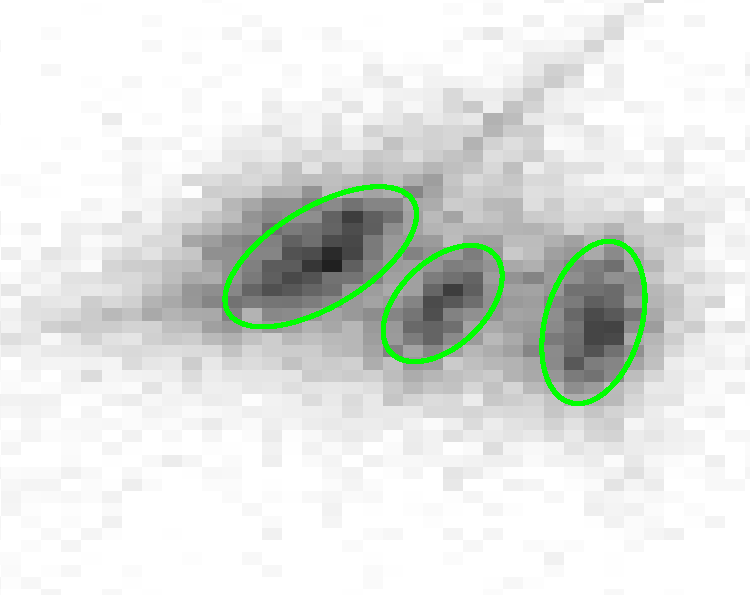
\includegraphics[width=.75\textwidth,height = 4.5 cm]{pf_punch2.pdf}
    \end{minipage}
    \begin{minipage}[c]{0.48\textwidth}
        \centering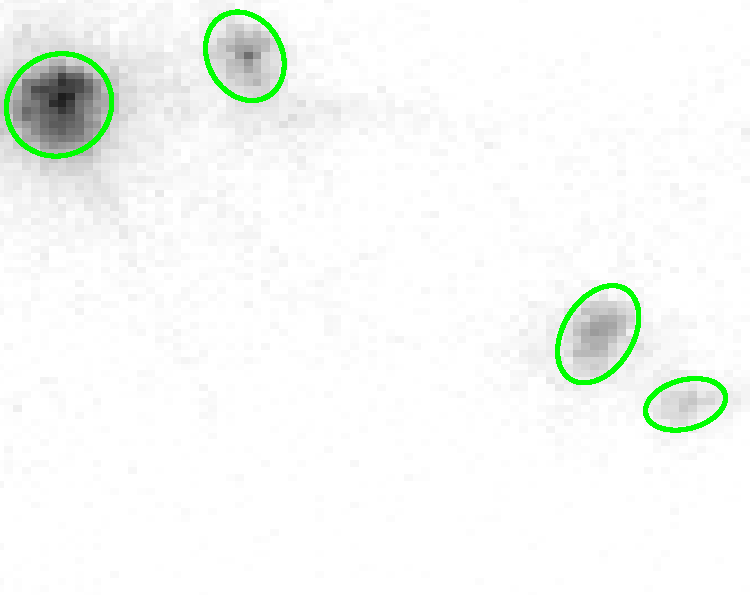
\includegraphics[width=.75\textwidth,height = 4.5 cm]{p_deff2.pdf}
    \end{minipage}
    \\
        \caption[Problémové detekce.]{Problémové detekce. Nalevo jsou laserové stopy blízko u sebe. Stopy je nutné od sebe oddělit. Na levém snímku jsou znázorněny výrazné rozdíly mezi velikostí a intenzitou stop. Je nutné použít víceúrovňový detektor. }
        \label{fig:Detekce}
\end{figure}

\newcommand\x{4}
\newcommand\xx{0,155}

\begin{figure}[htbp]
    \centering
    \begin{minipage}[c]{0.163\textwidth}
        \centering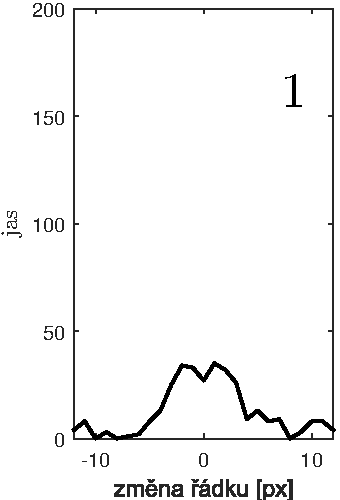
\includegraphics[height = \x cm,width = \textwidth ]{cut_1.pdf}
    \end{minipage}
    \begin{minipage}[c]{\xx \textwidth}
        \centering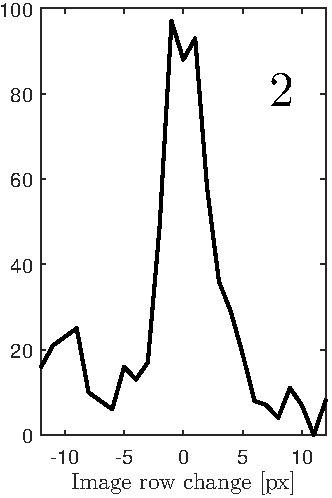
\includegraphics[height = \x cm,width = \textwidth]{cut_2.pdf}
    \end{minipage}
    \begin{minipage}[c]{\xx \textwidth}
        \centering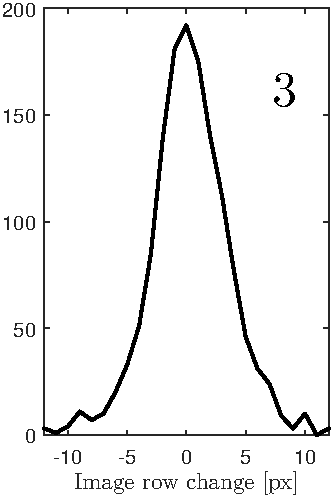
\includegraphics[height = \x cm,width = \textwidth]{cut_3.pdf}
    \end{minipage}
    \begin{minipage}[c]{\xx \textwidth}
        \centering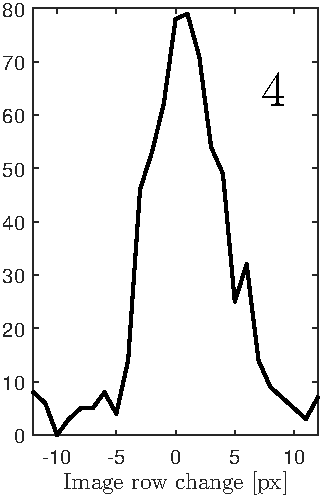
\includegraphics[height = \x cm,width = \textwidth]{cut_4.pdf}
    \end{minipage}
    \begin{minipage}[c]{\xx \textwidth}
        \centering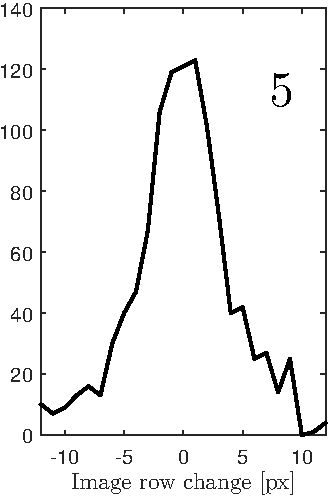
\includegraphics[height = \x cm,width = \textwidth]{cut_5.pdf}
    \end{minipage}
    \begin{minipage}[c]{\xx \textwidth}
        \centering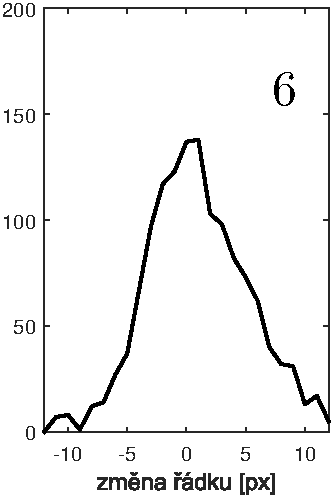
\includegraphics[height = \x cm,width = \textwidth]{cut_6.pdf}
    \end{minipage}
    \\
        \caption[Jasové řezy.]{Jasové řezy ve totožném sloupci obrazu. Řez protíná pixel s maximální hodnotou jasu ve stopě. Číslování řezů odpovídá indexům stop na obr. \ref{fig:Detekce}.}
        \label{fig:rezy}
\end{figure}

\section{Předchozí práce}

V předchozí práci \cite{Drapela} jsme neměli možnost detekovat stopy s nízkým jasem. Překrývající se svazky bylo nemožné oddělit.  

Bohatší pojetí problému se objevilo v Bodlákově práci \cite{Bodlak2005}. Snímek se prahoval více než jedním prahem, přičemž z oblastí nad prahem se sestavila stromová struktura a světelné stop se určily jako listy stromu s dostatečnou významností. Tento přístup je však pro svou výpočetní náročnost nepoužitelný pro snímky s rozlišením 2050$\times$2050, které máme k dispozici. 

Naše úloha detekce je velmi podobná detekci hvězd a galaxií v astronomických snímcích. V oblasti astronomie se hojně používá program s názvem Source Extractor \cite{SEXarticle}. Tento program má za sebou dlouholetý vývoj, je optimalizován z hlediska rychlosti a odzkoušený širokou veřejností. Tento software lze po naladění parametrů použít i pro náš případ. Nevýhodou však je, že nelze spustit v operačním systému Windows, který využíváme.  

Po testu různých detektorů jsme se rozhodli pro detekci laserových stop v obraze využít relativně nový přístup uveden J.Matasem et al. \cite{Matas} v roce 2002 - MSER detektor. 




\section{MSER (maximal stable extremal region) detektor}

MSER detektor hledá v obraze maximálně stabilní extrémní oblasti. Původně byl využit pro robustní nalezení korespondencí mezi dvěma snímky stejného objetu pořízených z různého místa a v současné době se používá v mnoha oblastech počítačového vidění.  

Princip spočívá v několikaúrovňovému prahování obrazu podle intenzity a nalezení spojitých oblastí, které jsou nad či pod prahovou hodnotou. Mezi úrovněmi jsou nalezeny korespondující oblasti a za MSER oblasti jsou označeny ty, jejichž velikost z předchozí úrovně se se zvyšující úrovní příliš nezměnila. 

Výhodou MSER detektoru je invariance vůči afinní transformaci intenzity a vůči změně měřítka, což umožňuje současnou detekci malých a velkých oblastí s různou intenzitou. Podle studie \cite{Comparison}, která porovnává MSER detektor s ostatními typy detektorů významných oblastí, dosáhl MSER detektor skvělých výsledků v detekci oblastí s vysokou hustotu a variabilní změnou velikosti. MSER detektor se tedy zdá být vhodným kandidátem pro detekci laserových stop v obraze.

\section{Implementace}

\subsection{Filtrace}
   Nejprve se pokusíme minimalizovat Poissonův šum v obraze. Šum redukujme konvolucí s maskou, která se skládá z prvků odpovídajících Gaussově funkci. Parametry filtru: velikost masky - \SI{3}{\px}, směrodatná odchylka $\sigma = 0.7$.

\subsection{Detekce} 
   %výstup MSER detektoru 
   Dalším krokem je detekce MSER oblastí ve filtrovaném snímku. MSER detektor je již implementován v prostředí MATLAB ve funkci \textit{detectMSERFeatures}. Pro aplikaci této funkce na snímek se světelnými stopami je třeba nastavit základní parametry detektoru. Mezi ně patří frekvence prahování snímku, maximální a minimální velikost MSER oblasti a dostatečná stabilita oblasti. 
   
   \begin{itemize}
   \item \textbf{Frekvecne prahování snímku.} - Určuje velikost kroku mezi prahovacími úrovněmi jasu (obr. \ref{fig:gaussIntersection}). Prahování se používá pro nalezení extremálních oblastí, na kterých se testuje stabilita.
   
   \item \textbf{Maximální a minimální velikost MSER oblasti.} 
   
   \item \textbf{Dostatečná stabilita oblasti.} - Velkost stabilní oblasti se po změně úrovně prahu intenzity příliš nemění. 
   \end{itemize}
   
\subsection{Okolí stínítka}
\label{sec:okoliStinitka}
	Okraj obrazu stínítka má tvar kružnice. Kružnici popisuje funkce
	
	\begin{equation}
	\left(x-x_0\right)^2 + \left(y-y_0\right)^2 = r^2\,,
	\label{eq:kruznice}
	\end{equation}
	kde $\left[x,y\right]$ je bod na kružnici, $\left[x_0,y_0\right]$ střed kružnice a $r$ poloměr. Je zřejmé, že k určení parametrů kružnice potřebujeme nalézt minimálně 3 body ležící na kružnici. 

	Úpravou rovnice \ref{eq:kruznice} dostaneme

	\begin{equation}
	x^2 -2\,x\,x_0 + x_0^2 + y^2 -2\,y\,y_0 + y_0^2 = r^2\,,
	\end{equation}
	\begin{equation}
	\begin{bmatrix}
    -2x &-2y &1 
	\end{bmatrix} \cdot 
	\begin{bmatrix}
    x_0 & y_0 & -r^2+x_0^2+y_0^2
	\end{bmatrix}^T = -\left(x^2+y^2\right)\,.
	\end{equation}


Polohu v obraze určujeme podle počtu pixelů v horizontálním (sloupec) a vertikálním (řádek) směru.
  
Body na kružnici nalezeme pomocí sečen. Sečny sestrojíme ve dvou řádcích snímku a nalezneme sloupce, ve kterých protínáme kružnici.  

Sestrojením sečny získáme jasový řez v celé šířce snímku. Fotonový šum jasu vyfiltrujeme konvolucí s Gaussovým filtrem. Velikost filtru volíme \SI{21}{\px} a směrodatnou odchylku $\sigma = 20$. 

Vyfiltrovaný jas oddělíme prahem. Práh určuje střední hodnota jasu v daném řezu. Nalezneme sloupce, kde je jas vyšší než prahové hodnota. Sloupec s minimálním resp. maximálním počtem pixelů určuje bod na kružnici.  

Každá sečna protíná kružnici ve dvou bodech, proto dostaneme celkem čtyři body na kružnici. Parametry kružnice určíme metodou nejmenších čtverců. 

Okolí stínítka poté definuje funkce 

\begin{equation}
	\left(x-x_0\right)^2 + \left(y-y_0\right)^2 > r^2\,.
	\label{eq:kruzniceOkoli}
	\end{equation}

\begin{figure}[htbp]
    \centering
    \begin{minipage}[c]{0.48\textwidth}
        \centering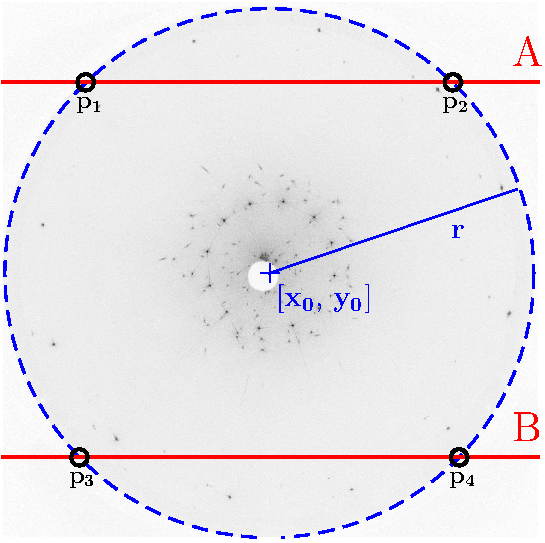
\includegraphics[width=\textwidth]{circleFit.pdf}
    \end{minipage}
    \begin{minipage}[c]{0.48\textwidth}
        \centering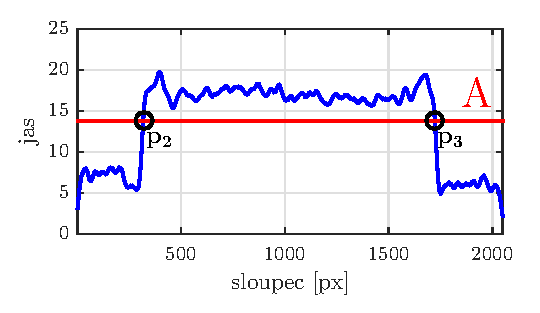
\includegraphics[width=\textwidth,height = 0.5\textwidth]{brigCutA.eps}\\
        
        \centering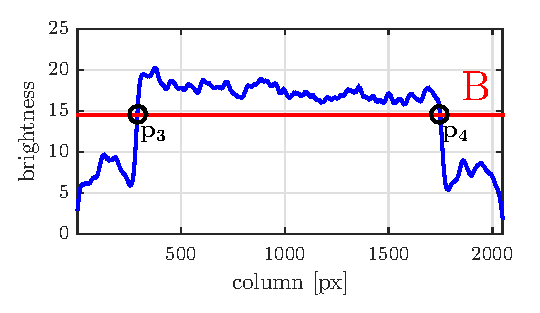
\includegraphics[width=\textwidth,height = 0.5\textwidth]{brigCutB.eps}
    \end{minipage}
    \\
        \caption[Detekce okolí stínítka.]{Jasové řezy \textit{A} a \textit{B}. Detekujeme body na kružnici $p_1$, $p_2$, $p_3$ a $p_4$. Metodou nejmenších čtverců odhadneme parametry kružnice $x_0$, $y_0$ a $R$.}
        \label{fig:CircleFit}
\end{figure}
	


\subsection{Pozadí snímku}
	V obraze nalezneme podstavec a okolí stínítka. Podstavec je specifický nízkou střední hodnotou jasu a jeho obraz je téměř ideální kruh. V seznamu MSER oblastí proto podstavec snadno nalezneme. Okolí stínítka již známe (kap. \ref{sec:okoliStinitka}).
	
	Velikost jasu v okolí stínítka nastavíme na hodnotu odvíjející se od střední hodnoty jasu snímku. Jas pixelů v oblasti podstavce nastavíme na střední hodnotu jasu pixelů v blízkém okolí podstavce.  
	
	Pozadí následně určíme konvolucí s Gaussovým filtrem. Tento filtr ignoruje vysoké změny jasu v obraze. Parametry filtru: velikost masky - \SI{201}{\px}, směrodatná odchylka $\sigma = 201$.
	
	Samotná konvoluce s tímto filtrem by s použitím standardní funkce \textit{conv2} byla příliš časově náročná, proto konvoluci provádíme efektivnějším způsobem, který využívá rozkladu masky filtru na singulární čísla.
	
\begin{figure}[htbp]
    \centering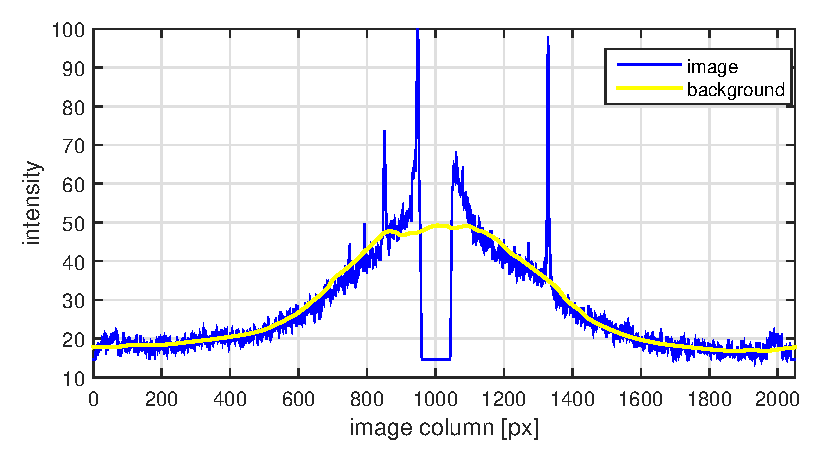
\includegraphics[width=.8\textwidth]{image_rust2.eps}
     \caption[Filtrace pozadí.]{Filtrace pozadí v HDR snímku znázorněná v řádku obrazu protínajícím obraz podstavce na kámen.}
        \label{fig:pozadi}
\end{figure}
	      
\subsection{Odstranění nežádoucích detekcí}

Výstupem detektoru je soubor MSER oblastí. U výrazné světelné stopy dostaneme data ve formě pyramidy MSER oblastí podle jednotlivých úrovní intenzity. 

MSER detektor však najde nejen oblasti s výrazně vyšší intenzitou, ale i oblasti s nižší intenzitou než okolí. Ty je třeba vyřadit, protože nereprezentují světelnou stopu, kterou hledáme. 

K odstranění nežádoucích detekcí použijeme následující postup. 

\begin{enumerate}
\item Od filtrovaného snímku odečteme pozadí.

\item Ve vzniklém snímku vypočítáme střední hodnotu jasu MSER oblastí. 

\item Pokud je střední hodnota jasu záporná, MSER oblast odstraníme.  
\end{enumerate}
 	      

\section{Určení parametrů svazku}
\label{sec:beam parameters}
Základním parametrem svazku je směr šíření popsaný azimutem a elevací. Směr šíření svazku snadno dopočítáme, pokud nalezneme jeho obraz. Pozici světelné stopy v obraze lze určit jako polohu pixelu s maximálním jasem v detekované oblasti. Šum v obraze ale situaci komplikuje. Z obr. \ref{fig:rezy} ale vidíme, že pixel s maximálním jasem nemusí vždy určovat pozici dopadu a navíc nemusí být unikátním maximem.

Laserové svazky se v reálném případě rozptylují. Kvůli různé rozbíhavosti svazků nejsme schopni určit údaje o ploše a intenzitě jejich obrazu. Určujeme pouze velikost zářivého toku svazku, kterou jsme schopni při nízkém rozptylu spolehlivě vypočítat.   

V okolí obrazu svazků jsou patrné ocásky. Detekce ocásků a jejich klasifikace je popsána v samostatné kapitole \ref{sec:tails}.

Rozbíhavost svazků nemusí být ve všech směrech stejná. Na stínítku tak svazky tvoří stopy různých tvarů. Tvar stopy definujeme pomocí 3 parametrů.

\subsection{Základní parametry}

Máme detekované MSER oblasti. Nalezneme průniky oblastí a sestavíme stromovou strukturu. Kořenem stromu bude oblast s největší plochou a postupně se budou přidávat oblasti menší. Princip je patrný z 2D pohledu na prahovací úrovně MSER detektoru v obr. \ref{fig:gaussIntersection}, kde vidíme i princip tvorby stromu. Výsledkem bude řada stromů s různým počtem listů. Počet všech listů určuje počet detekovaných stop v obraze.

\begin{figure}[htbp]
    \centering
	\begin{minipage}[c]{0.78 \textwidth}
    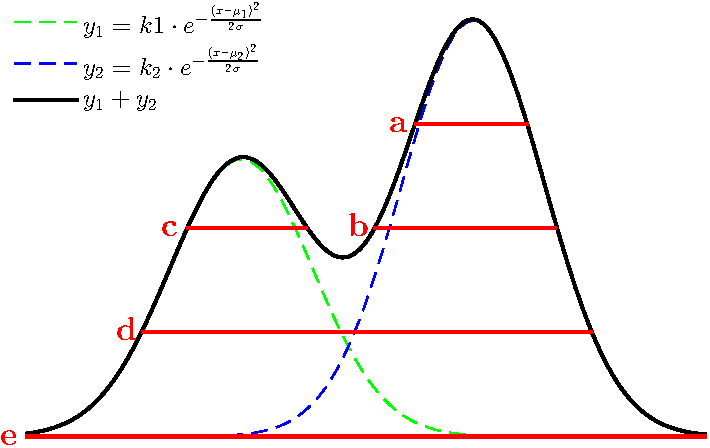
\includegraphics[width=\textwidth]{gaussIntersection.pdf}
    \end{minipage}
    \begin{minipage}[c]{0.16 \textwidth}
    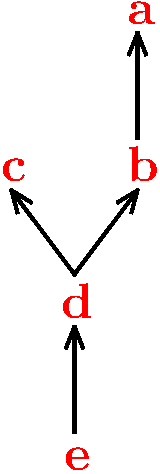
\includegraphics[width=\textwidth]{treeGauss.pdf}
    \end{minipage}
    
    
     \caption[]{Ilustrace překrytí stop v 2D řezu. Výsledná charakteristika je součtem dvou gaussových funkcí. Červeně jsou zakresleny prahovací úrovně MSER detektoru. Vlevo vidíme stromovou strukturu MSER oblastí a-f. Kořenem stromu je vrstva \textbf{e}. Vrstva \textbf{d} je jediný vnitřní uzel stromu. Listy představují vrstvy \textbf{c} a \textbf{a}. Důležité jsou podstromy \textbf{e}$\rightarrow$\textbf{d}, \textbf{c}, \textbf{b}$\rightarrow$\textbf{a}.}
        \label{fig:gaussIntersection}
\end{figure}

Cíleně prohledáváme jednotlivé stromy a nalézáme uzly, ze kterých počítáme parametry svazků.

\begin{itemize}
	\item \textbf{Azimut a elevace} - Pozici dopadu světelné stopy určíme jako střed eliptické aproximace oblasti odpovídající listu stromu. Transformací z \cite{Drapela} získáme azimut a elevaci.
	
	\item \textbf{Zářivý tok} - 
	Od filtrovaného snímku odečteme pozadí (obr. \ref{fig:pozadi}) a získáme snímek, ze kterého budeme odečítat intenzitu pixelů. Algoritmus výpočtu zářivého toku je následující:
	\begin{enumerate}
	\item $t_0$ = původní strom; $i = 0$; $q = 0$; $n_0$ = počet listů v $t_0$;
	
	\item Ve stromu $t_i$ nalezneme podstromy $\tau_1,\dots,\tau_n$ maximální velikosti bez vnitřních uzlů stromu $t_i$ a obsahující jeden list stromu $t_i$.  
	
	\item Nalezneme křeny $\xi_1,\dots,\xi_n$ podstromů $\tau_1,\dots,\tau_n$. Kořeny odpovídají oblastem s množinou pixelů $\mathbb{M}_{q+1},\dots,\mathbb{M}_{q+n}$.
	
	\item Pokud $i = 0$ vypočítáme zářivý tok 
	
	\begin{equation}
	\phi_{e_j} = \frac{\sum_{k\in\mathbb{M}_j} I_k}{N_j}\,,\hspace{2cm} j\in\lbrace1,\dots,n_0\rbrace
	\end{equation}
	kde $I_k$ je jas pixelu $k$ ve snímku a $N_j$ je počet pixelů v množině $\mathbb{M}_j$. Index $j$ odpovídá indexu stopy ve stromu $t_0$.\\
	
	Pokud $i > 0$ nalezneme množiny $\mathbb{P}_1,\dots,\mathbb{P}_n$. $\mathbb{P}_l$ je množina indexů listů, které jsou v $t_0$ potomkem uzlu $\xi_l$, kde $l\in {1,\dots,n}$. Zářivý tok stop upravíme.  
	 \begin{equation}
	\phi_{e_j} = \frac{\phi_{e_j}}{\sum_{q\in \mathbb{P}_l}\phi_{e_q}}\frac{\sum_{\lbrace k\in\mathbb{M}_{q+l}\cap\lbrace \mathbb{M}_1^c \cup \mathbb{M}_2^c \cup \dots \cup \mathbb{M}_q^c \rbrace\hspace{1.5mm}|\hspace{1.5mm} \lbrace1,2,\dots,q\rbrace = \mathbb{P}_l \rbrace} I_k}{N_{q+l}} + \phi_{e_j}\,.\hspace{0.5cm} j\in \mathbb{P}_l
	\end{equation}
	
	\item $i = i+1$; $q = q+n$;
	\item Pokud $n \neq 1$ odstraníme podstromy $\tau_1,\dots,\tau_n$ z grafu $t_{i-1}$, získáme strom  $t_i$ a opakujeme od kroku $2$. 
	
\end{enumerate}	
	\item \textbf{Tvar} -  Pro každou MSER oblast je určena elipsa, která uzavírá danou oblast. U této elipsy lze určit orientaci a velikost hlavních poloos. 
	
	Každé stopě odpovídá jeden list stromu. Nalezneme cestu $\mathcal{C}$, která je cestou od kořene k listu. 	
	
	Orientace je určena jako medián orientací elips všech MSER oblastí v cestě $\mathcal{C}$. Velikosti hlavních poloos jsou určeny podle MSER oblasti, která je uprostřed cesty $\mathcal{C}$.		
		
\end{itemize}

	
	
	
\subsection{Detektor ocásků}
\label{sec:tails}
	Se znalostí směru a velikosti ocásků detekovaných svazků dostáváme nové informace, které nohou přispět k jejich správnému párování se svazky z matematického modelu kamene.
	
	Ve snímaném obraze nelze rozpoznat všechny vznikající ocásky, ale pouze ty s dostatečně velkou intenzitou.

	Princip detektoru ocásků zjednodušeně spočívá v převodu okolí stopy do polárních souřadnic (vzdálenost $\rho$ a úhel $\phi$) a nalezení oblastí úhlů, ve kterých je patrný výrazný vzestup intenzity oproti okolí. Takovéto oblasti jsou typicky důsledkem přítomnosti ocásků o obraze a lze tímto způsobem ocásky detekovat. 
	
	 U rozvinutí do polárního grafu si však musíme všimnout překážek, které komplikují detekci ocásků.  
	 \begin{itemize}	 	
	 	\item V blízkém okolí jedné stopy se může nacházet další stopa. V polárním grafu se tato blízká stopa jeví jako ocásek a dochází k falešné detekci.	
	 	\item Stopy a ocásky jsou v obraze různě velké. Je třeba efektivně určovat vzdálenost $\rho$ do které budeme převádět okolí stopy do polárního grafu. Pokud zvolíme malé $\rho$ nepokryjeme oblast, kde se vyskytují ocásky a velké $\rho$ zvýší časovou náročnost výpočtu.   	
	\end{itemize}
	
	Elegantní řešení přináší použití MSER detektoru, pomocí něhož získáme vymezení oblasti a tím i vzdálenosti $\rho$, kde se stopa i s ocásky nachází. Se znalostí oblastí náležící jednotlivým stopám jsme schopni od sebe stopy částečně oddělit a redukovat množství falešných detekcí. Na druhou stranu sousední stopa muže ležet na pozici ocásku a odstraněním sousední stopy odstraníme současně i ocásek, který prozatím nejsme schopni v případě překrytí oddělit. Vzhledem k rozmanitosti stop, co do velikosti, intenzity, množství a tvaru ocásků apod. není jednoduché stopu matematicky modelovat. Pokud by se podařilo vytvořit dostatečně přesný kompaktní model stopy, je možné uvažovat o situaci, kdy budeme schopni od sebe separovat překrývající se stopy a ocásky. 
	
 Pro znázornění postupu a mezivýsledků jsme si vybrali laserovou stopu (obr.\ref{fig:mark_tail}), která v obraze nekoliduje s další výraznou stopu. Zvolená stopa vznikla dopadem laserového svazku typu ...!!doplnit(až budou popsány všechny třídy svazků)!!.... V obraze jsou patrné čtyři ocásky různě intenzity. 
	

	\begin{figure}[htp]
	\centering
	\begin{minipage}[c]{0.4\textwidth}
	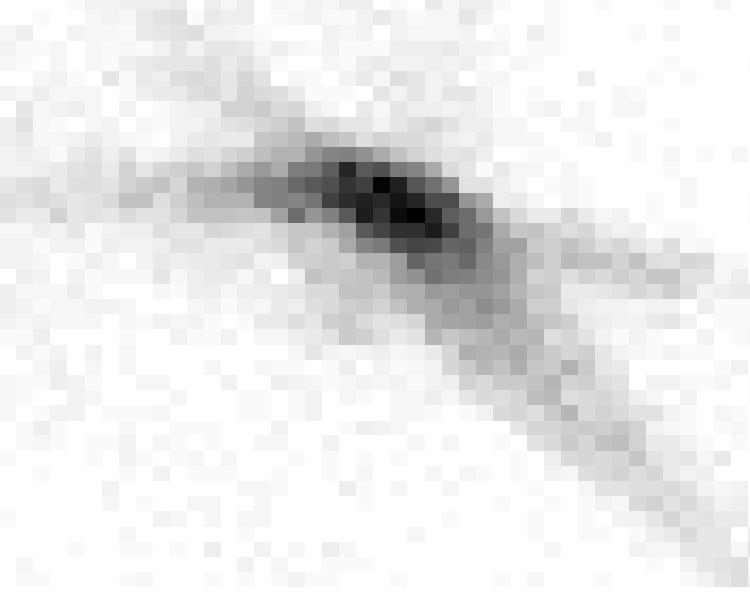
\includegraphics[width=\textwidth]{figures/tail07.pdf}
	\end{minipage}
	\begin{minipage}[c]{0.4\textwidth}
	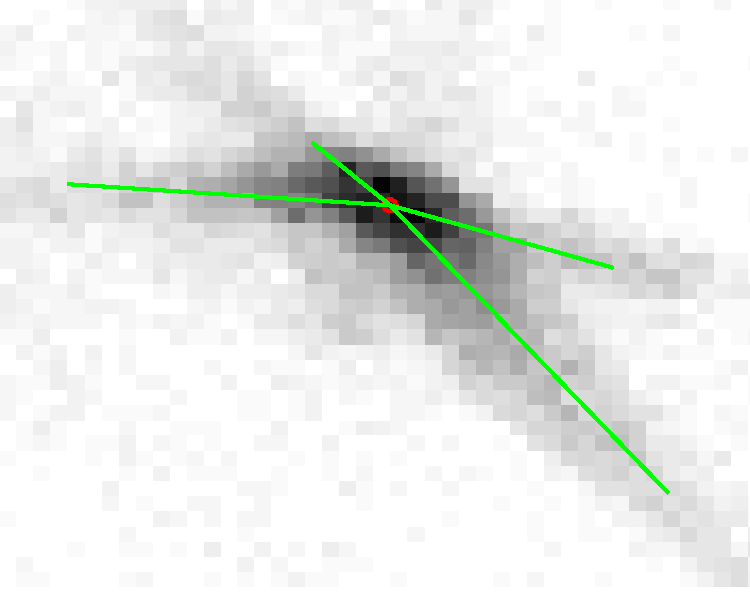
\includegraphics[width=\textwidth]{figures/tail08.pdf}
	\end{minipage}\\
	\begin{minipage}[c]{0.4\textwidth}
	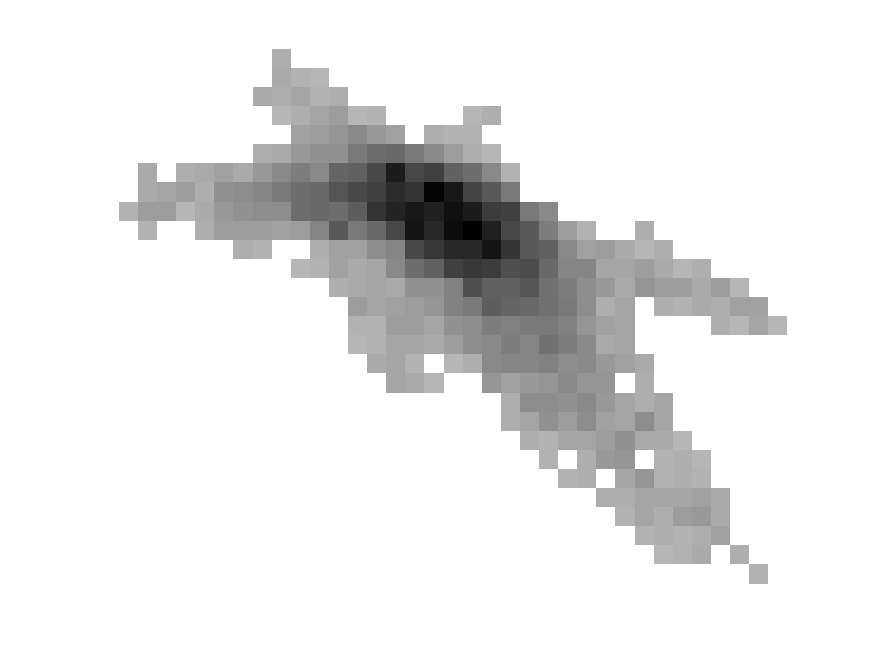
\includegraphics[width=\textwidth]{figures/tailex01.pdf}
	\end{minipage}
	\begin{minipage}[c]{0.4\textwidth}
	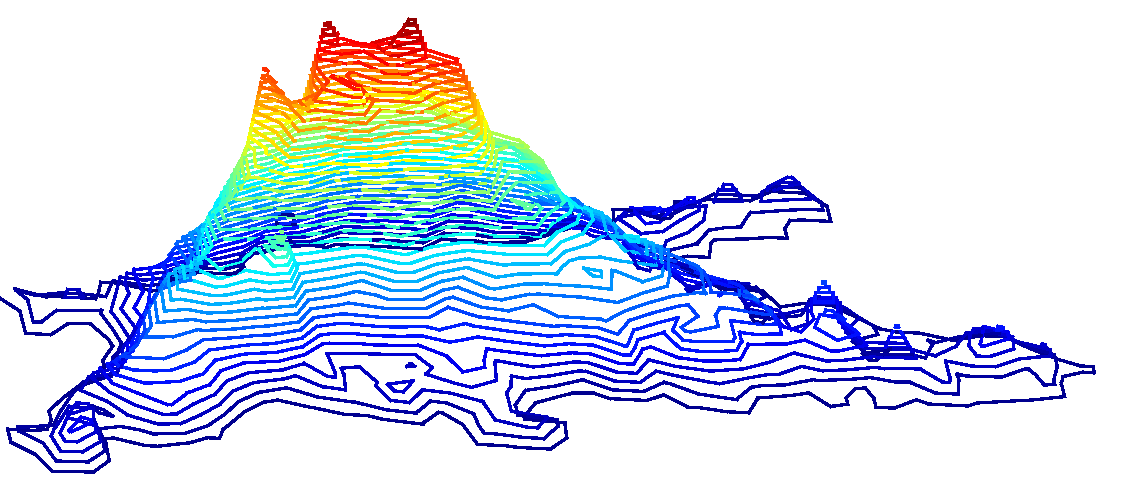
\includegraphics[width=\textwidth]{figures/tailex02.pdf}
	\end{minipage}
	
	\caption[Detektor ocásků - laserová stopa.]{Zvolená laserová stopa k ilustraci algoritmu detektoru ocásků. Stopa vznikla dopadem svazku typu $\dots \dots$ na stínítko. V měřicí soustavě byl přitom umístěn kámen typu \textit{VIVA $12$} s odstínem \textit{Crystal} a průměrem \SI{4.8}{\milli\meter}. Snímek vpravo nahoře znázorňuje výřez stopy ze snímaného obrazu. Můžeme zde pozorovat čtyři ocásky s různými vlastnostmi. Vlevo nahoře je výsledek detekce popsané níže. Obrázek vpravo dole ukazuje MSER oblast a poslední obrázek znázorňuje 3D pohled na zkoumanou stopu.}
	\label{fig:mark_tail}
	\end{figure}


Jednotlivé kroky algoritmu: 
	\begin{itemize}
	\item Vybereme stopu, u které chceme identifikovat ocásky a ze snímku vybereme oblast (obr.\ref{fig:mark_tail}), která náleží zkoumané stopě. 
	
	\item Po odečtení okolního šumu $z_{noise}$ prahujeme intenzitu pixelů stopy $2$krát střední hodnota intenzity $z_{mean}$. Pixely s intenzitou vyšší než zvolený práh nastavíme intenzitu odpovídající prahové hodnotě a posuneme $z_{noise}$ na hodnotu $z_{mean}$ tak, že ke všem pixelům přičteme intenzitu $z_{mean}$. Důvodem tohoto kroku je snaha odstranit nežádoucí vlastnosti velkého šumu v hodnotách intenzity v blízkém okolí "těžiště" stopy a také to, že se chceme zvětšit relativní příspěvek pixelů s nižší intenzitou do součtového kritéria \ref{eq:Isuma}.   
	
	\item Stopu s velikostí okolního šumu $z_{mean}$ převedeme do polárních souřadnic ($\rho$, $\phi$). Intenzitu $I_{pol}$ v polárním grafu $I_{pol} = f(\phi,\rho)$ určujeme pomocí bipolární interpolace, která pro větší efektivitu vynechává oblasti mimo oblast stopy, kde $I_{pol} = 0$. Důležitým parametrem při interpolaci je velikost vzorkování $f_{\phi}$ úhlu $\phi$ resp. vzorkování $f_{\rho}$ vzdálenosti $\rho$ . Experimentálně jsme zvolili $f_{\phi} = \SI{3}{\degree}$ a $f_{\rho} = \SI{1}{\px}$. Interpolaci počítáme v intervalech  $\phi \in \left\langle 0,2\pi \right\rangle$ a $\rho \in \left\langle 1,\rho_{max} \right\rangle$, kde $\phi_{max}$ je maximální vzdálenost všech pixelů v oblasti stopy od její pozice.  
	
	\begin{figure}[htbp]
    \centering
    \begin{minipage}[c]{0.48\textwidth}
        \centering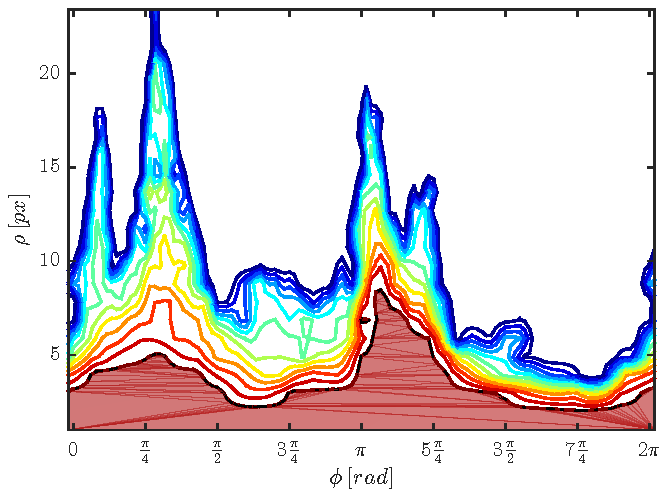
\includegraphics[width=.98\textwidth]{tailex03.pdf}
    \end{minipage}
    \begin{minipage}[c]{0.48\textwidth}
        \centering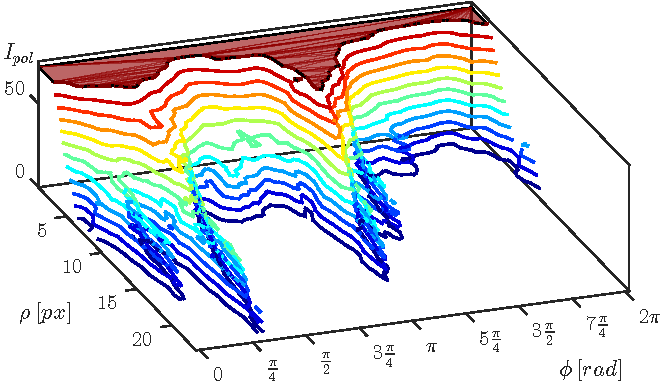
\includegraphics[width=.98\textwidth]{tailex04.pdf}
    \end{minipage}
    \\
        \caption[Detektor ocásků - polární graf.]{Dva pohledy na intenzitu okolí stopy převedené do polárního grafu $I_pol$ zobrazené pomocí vrstevnic.}
        \label{Detekce}
\end{figure}
	
	\item Provedeme součet intenzit $I_{pol}$ pro jednotlivé úhly $\phi$ od minimální do maximální vzdálenosti $\rho$ a získáme závislost $I_\phi = f(\phi)$, kde  
	
	\begin{equation}
	I_{\phi_i} = \sum_{j = 1}^{\rho_{max}} I_{pol}\left(i,j\right)\,. \hspace*{2cm} i \in \left\lbrace 0, \frac{3}{180}\pi, \dots \,,2\pi \right\rbrace
	\label{eq:Isuma}
	\end{equation}
	Následně na $I_{\phi}$ aplikujeme kubickou interpolaci sousedních hodnot s $5$krát citlivějším vzorkováním $f_{\phi_2} = \frac{f_{\phi}}{5}$ a rozšíříme rozsah $\phi$ na $\phi \in \left\langle -\frac{\pi}{2},\frac{5}{2}\pi \right\rangle$. 
	
	\item Graf závislosti $I_\phi = f(\phi)$ filtrujeme konvolucí s gausiánem $g(x)$ se směrodatnou odchylkou $\sigma = 3$ a získáme referenční závislost $I_{filt}$.
	
	\begin{equation}
		g(x) = \frac{1}{\sqrt{2\pi} \cdot \sigma}e^{-\frac{x^2}{2\sigma^2}}\,.
	\end{equation}
	
	\begin{figure}[htbp]
    \centering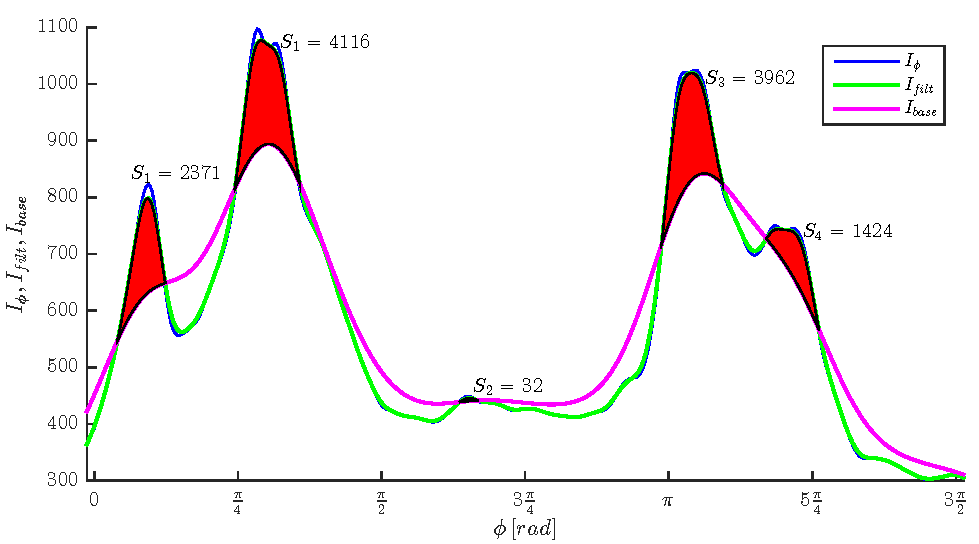
\includegraphics[width=\textwidth]{figures/tailex05.pdf}
     \caption[Detekce ocásků - zpracování polárního grafu.]{Grafické vysvětlení funkce algoritmu pro detekci ocásků. }
    \label{fig:tailSumGraph}
	\end{figure}
	
	\item Na graf $I_{filt}$ následně opakovaně aplikujeme konvoluci, tentokrát s gausiánem $g(x)$ s vyšší směrodatnou odchylkou $\sigma = 8$, abychom získali základnu $I_{base}$, kterou budeme porovnávat se signálem $I_{filt}$.
	
	\item Nalezneme souvislé oblasti $\mathcal{R}_1, \dots , \mathcal{R}_n$, kde graf $I_{filt}$ má větší hodnotu než $I_{base}$ a sečteme rozdíly $I_{filt}$ a $I_{base}$ v jednotlivých vzorcích. Velikost součtu $S_1, \dots , S_n$ závisí na vzorkovací frekvenci $f_{\phi_2}$.
	
	\begin{equation}
	S_i = \sum_{\phi_j \colon \phi_j \in \mathcal{R}_i}I_{filt}(\phi_j)-I_{base}(\phi_j)\,. \hspace*{2cm} i \in \left\lbrace 1, 2, \dots \,, n \right\rbrace
	\label{eq:Rsuma}
	\end{equation}
	
	\item Za ocásek uvažujeme oblast $\mathcal{R}_i$, kde je součet $S_i$ větší než prahovací úroveň $s_{th}$ (pro $f_{\phi_2}$ je $s_{th} = 500$). Směr ocásku $\varphi$ je určen jako úhel, ve kterém je graf $I_{filt}$ v dané oblasti maximální a velikost ocásku $\varrho_i$ určuje $\rho_{max}$ a poměr součtu $S_i$ k maximálnímu v pro danou stopu.  
	
	\begin{equation}
	\varphi_i = \argmax_{\phi_j \colon \phi_j \in \mathcal{R}_i}I_{filt}(\phi_j) \,, \hspace{1cm} \varrho_i = \frac{S_i}{\max_{j \in 1,\dots , n}S_j}\rho_{max}\,.
	\label{eq:tail_params}
	\end{equation}
		
	\begin{figure}[htbp]
    \centering
    \begin{minipage}[c]{0.48\textwidth}
        \centering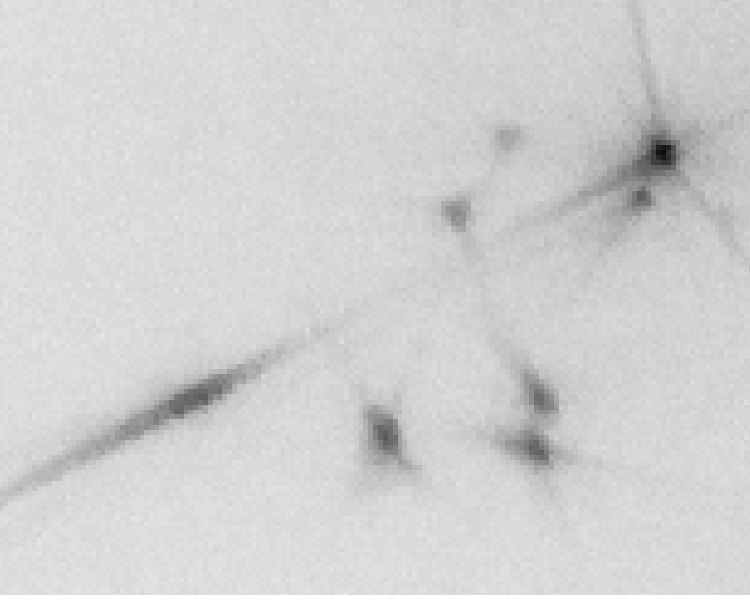
\includegraphics[width=.98\textwidth]{tail01.pdf}
    \end{minipage}
    \begin{minipage}[c]{0.48\textwidth}
        \centering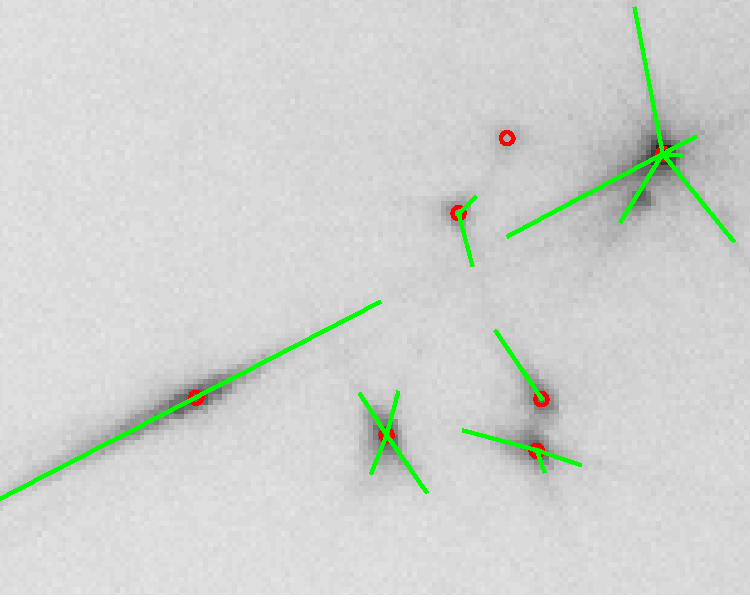
\includegraphics[width=.98\textwidth]{tail02.pdf}
    \end{minipage}
    \\
        \caption[Detektor ocásků - příklad detekce.]{Ukázka funkce detektoru ocásků na vybraném vzorku z obrazu. }
        \label{Detekce}
\end{figure}


	
	
\end{itemize}	   
	
	

\section{MSER detector configuration parameter list}	
	Here is a list of the configuration parameters used for beam detection setting. All of them can be used with their default values. This description of the parameters can be usefull for understanding the algorithm or debugging.
	
\begin{center}


\begin{tabular}{l|l|p{8cm}}
    \textbf{Name} 		& \textbf{Default} & \textbf{Description} \\ \hline \hline 
    \textit{BackgroundFilt}	    	& $201$ 	& Size of Gaussian filter mask used for background estimation. \textit{Sigma} of mask is equal to \textit{BackgroundFilt} \\ \hline
    \textit{BackgroundKMean}    	& $0.15$	& $BackgroundKMean \times mean(image)$ is added to background estimation. \\ \hline
    \textit{ComputeAllLayers}   	& $1$		& $1$ - Divide all layers in marks variable calculation. $0$ - Calculate only with upper layers. \\ \hline
    \textit{ComputeTails}   		& $ 1 $		& $1$ - Tails of marks are computed. It takes some time. $0$ - No tails. Faster.\\ \hline    
    \textit{CleanerAxisRatio}   	& $ 10 $	& MSER regions with upper axis ratio are deleted. \\ \hline
    \textit{CleanerFilterSigma}  	& $ 5 $		& \textit{Sigma} of filter mask in image blurring. \\ \hline
    \textit{CleanerFilterSize}   	& $ 31 $	& Size of filter mask in image blurring.\\ \hline
	\textit{CleanerMean}    		& $ 0.035 $ & Regions with peak where difference of mean of surrounding
intensity is lower than $CleanerMean \times mean(image)$ are deleted. \\ \hline
    \textit{CleanerSumWide} 		& $ 5 $		& Size of surrounding in cleaning process.  \\ \hline
    \textit{FilterSigma}    		& $ 0.7 $	& \textit{Sigma} of niose reducing filter mask. \\ \hline
    \textit{FilterSize} 			& $ 3 $		& \textit{Size} of niose reducing filter mask.\\ \hline 
    \textit{MSERMaxAreaVar} 		& $ 0.9 $	& This value specifies the step size between intensity threshold levels used in selecting extremal regions while testing for their stability. Decrease this value to return more regions.\\ \hline
    \textit{MSERRegion} 			&$[2\,,\, 14000]$& Two-element vector, [minArea maxArea], which specifies the size of the regions in pixels. This value allows the selection of regions containing pixels between minArea and maxArea, inclusive.\\ \hline
    \textit{MSERThresh} 			& $ 1.2 $	& Increase this value to return a greater number of regions at the cost of their stability. Stable regions are very similar in size over varying intensity thresholds.\\ \hline
    \textit{SurroundThres}   		& $ 0.8 $	& Multiple of $mean(image)$ where surrounding intensity is moved.   \\ 
\end{tabular}

\end{center}

%\clearpage